This chapter introduces the fundamental concepts related to the developments presented in this thesis. The major areas introduced are: Epigenetics, Genetics, (Epi)Genomic data analysis.


\section{Epigenetics alterations}
\subsection{DNA methylation}
\section{Histone modifications}

\section{Genetics alterations}


\section{(Epi)Genomic data analysis}

\subsection{Integrative analysis}
Often the onset and progression of cancerous diseases is linked to the aberrant function of proteins and alterations in gene expression, which has led research in genetics in search of the molecular alterations responsible for such aberrant behavior.
Among the types of alterations genetic and epigenetic
that can impact gene function are, gene copy number
(CN), DNA methylation, single nucleotide variations (SNV), and indels (small insertions and
deletions).
These variantions can have a direct affect by modifying
 function of the gene product, for example a
indel in a coding region, or a indirect affect such as
the modification of regulatory regulatory regions
 which can interfere
 with gene expression by inhibiting transcription \cite{thingholm2016strategies}.

Furthermore, recent technological developments have enabled the creation of genome-wide data for multiple types of variations.
Although individual analyzes of these variations helped  increasing knowledge of the genome and of complex
disorders, integrative analyses that evaluate cancer transcriptome data in the context of other data sources are often capable of extracting deeper biological insight from the data \cite{rhodes2005integrative}.

In this section we will highlight several integrative  approaches, including meta-analysis for extracting robust profiles from independent data sets, enrichment analysis for identifying coordinately regulated functional gene modules, protein interaction networks for detecting interaction complexes deregulated in cancer, transcriptional networks for inferring regulatory mechanisms in cancer and analyses of model system profiles with human tumor profiles for inferring activity of oncogenic pathways.

\subsubsection{Functional enrichment analysis of cancer signatures}

A \sigla{GSEA}{gene set enrichment analysis} or  functional enrichment analysis is a method to identify classes of genes or proteins that are over-represented in a large set of genes or proteins, and may have an association with disease phenotypes.
This type of analysis integrates  differentially expressed genes identified by a  \sigla{DEA}{differential expression analysis} and integrating these information with external functional information is necessary for interpreting and summarizing large cancer signatures.
Most approaches use external annotation databases such as Gene Ontology which is a database of controlled vocabulary gene annotations describing the biological processes, molecular functions and cellular localizations of genes as a resource for enrichment analysis in cancer signatures.

Let $L$ be a  list of genes ranked by their differential expression between the classes, the goal of GSEA is to determine whether members of a gene set $S$ tend to occur toward the top (or bottom) this list,  which might correlated with the phenotypic class
distinction \cite{subramanian2005gene}.

\subsubsection{Protein interaction networks and cancer signatures}

A major objective of systems biology is to organize molecular interactions as networks \cite{vinayagam2014integrating}. \sigla{PPIs}{Protein-protein interactions } are essential to almost every process in a cell, and they are not only crucial for understanding cell physiology in normal and disease states since the disruption of protein-protein interactions may result in disruption of the cell component or process to which they contribute, compromising the cell viability or even leading to cell death, but also for the drug development, since drugs can affect PPIs \cite{PPIs,alzate2009neuroproteomics}.
These interaction are represetented as \sigla{PPIN}{Protein-protein interaction networks}, a mathematical representations of the physical contacts between proteins in the cell.
The totality of PPIs that happen in a cell, an organism or a specific biological context is called interactome.

 A detailed human interactome network that captures the entire cellular network is invaluable in interpreting cancer signatures, allowing one to infer activated subnetworks and specific proteins that are most important to a subnetwork. For example, for a given set of overexpressed proteins in the same subnetwork, one specific protein thart interacts with the entire subnetwork might be the key to control the expression the entire subnetwork.

 A lot of this information is available through molecular interaction databases such as IntAct (\burl{ http://www.ebi.ac.uk/intact}) \cite{orchard2013mintact}.

\subsubsection{Transcriptional targets and cancer signatures}

Similar to the Protein-protein interaction networks, global transcriptional networks, which defines directional pathways (i.e. which gene actives are activated by a given gene), have the potential to improve the interpretation of cancer signatures. For example, if the targets of all transcription factors  were known, then one could easily infer which transcription factors must be activated in a tumor to yield the observed cancer signature. With that information, it is possible to reduce a complex cancer signature to a small number of activated transcriptional factors which will be potencial therapeutic targets.

The identification of transcription factor-binding sites (TFBSs) is done using high throughput experimental methods  such as ChIP-Chip and  \sigla{ChIP-seq}{ChIP-sequencing} which identifies a region of 100–1000
base pairs (b.p.) in which the TFBS
(typically 9-15 b.p.) resides \cite{jayaram2016evaluating}.
In-silico  sequence-based methods were develop to predicted TFBSs. These methods scans a DNA sequence of interest
with a \sigla{PWM}{position weight matrix},a $4 x n$ matrix of
scores for each of the 4 bases across each position in the
binding motif, for a transcription factor of interest and perform a pattern-matching.
PWM models can be obtained from a number of resources including the the open access database JASPAR \cite{portales2009jaspar}, HOCOMOCO \cite{kulakovskiy2013hocomoco} and HOMER \cite{heinz2010simple}. Among the existing  software that scans a sequence database for individual matches to each of the motifs are \sigla{FIMO}{Find Individual Motif Occurrences} \cite{grant2011fimo}, HOMER \cite{heinz2010simple} and PATSER \cite{turatsinze2008using}.

\subsubsection{Human Epigenomes}
The human body contains  more than 200 different cell types
each one has an identical copy of the genome but expresses a distinct set of genes, due to their epigenome which in each cell regulates gene expression in a number of ways - by organizing the nuclear architecture of the chromosomes, restricting or facilitating transcription factor access to DNA, and preserving a memory of past transcriptional activities \cite{rivera2013mapping}.
The integrative analysis of epigenomic maps, which references to the collection of DNA methylation state and covalent modification of histone proteins along the genome \cite{bonasio2010molecular}, has been shown to be important in the study of the gene regulatory programs \cite{gifford2013transcriptional,hawkins2010distinct,rada2012epigenomic}.


\bgroup
\def\arraystretch{2.0}%  1 is the default, change whatever you need
\begin{table}[]
\centering
\small
\caption[Histone and epigenomic marks]{Core set of five histone modification marks and other epigenomic marks}
\label{histonemarks}
\begin{tabular}{lp{8cm}}
\toprule
 \textbf{Histone marks}   & \textbf{Role} \\ \toprule
 Histone H3 lysine 4 trimethylation (H3K4me3)  & Promoter regions \cite{heintzman2007distinct,bernstein2005genomic} \\
 Histone H3 lysine 4 monomethylation (H3K4me1) & Enhancer regions \cite{heintzman2007distinct}  \\
 Histone H3 lysine 36 trimethylation (H3K36me3) & Transcribed regions  \\
 Histone H3 lysine 27 trimethylation (H3K27me3) & Polycomb repression \cite{bonasio2010molecular}  \\
 Histone H3 lysine 9 trimethylation (H3K9me3) & Heterochromatin regions \cite{peters2003partitioning} \\
 Histone H3 acetylated at lysine 27 (H3K27ac)  &  Increase activation of genomic elements \cite{heintzman2009histone,rada2011unique,creyghton2010histone} \\
 Histone H3 lysine 9 acetylation  (H3K9ac)  & Transcriptional activation \cite{nishida2006histone} \\
 DNase hypersensitivity &  Regions of accessible chromatin \cite{thurman2012accessible}\\
 DNA methylation & Repressed regulatory regions \cite{cedar2009linking,moore2013dna}\\  \bottomrule
\end{tabular}
\end{table}
\egroup
%The goal is to discover epigenomic states and aid in understanding
%“non-coding” genomic elements in an unbiased and biologically meaningful way

%The most popular and widely used of these machine learning methods is ChromHMM

\subsection{Statistical analysis}

\subsubsection{Hypothesis Testing}

Human genetic studies aims to identify if a phenotype is related to the genotypes
at various loci, that is, if genetic variations have an influence on risk of
disease or other health-related phenotypes.
Statistical analysis is a crucial to present the findings in an
interpretable and objective manner \cite{sham2014statistical}.

The most popular hypothesis testing approach used to test if
genotypes and phenotypes are related  is the frequentist significance testing approach.
This is a classical approach that involves setting up two competing hypothesis: a
null hypothesis ($H_0$\simbolo{H_0}{Null hypothesis}) and an alternative hypothesis ($H_1$\simbolo{H_1}{Alternative hypothesis}).

Computing the statistical significance can be done using a one-tailed or a two-tailed test.
A two-sided test is appropriate to evaluate both direction of the test, for example,
is the estimated value smaller or higher than the reference, which acctualy test if the
 estimated value is different from the reference.
A one-sided test is  is appropriate to evaluate only one direction of the test,
for example, is the estimated v alue smaller than the reference.
An example in genetic studies for a two-sided test would be $H_0$
hypothesis that genotypes has no effect on the phenotypes
while the $H_1$ hypothesis is that there is a effect.
Table \ref{hypothesis-tests} shows other examples.

% Please add the following required packages to your document preamble:
% \usepackage{booktabs}
\begin{table}[h!]
\centering
\caption[Hypothesis tests]{Example of three hypothesis tests about the population mean $\mu$. In genetics it could be the mean level of expression of a gene.}
\label{hypothesis-tests}
\begin{tabular}{@{}lll@{}}
\toprule
\multicolumn{1}{c}{\textbf{Type}} & \multicolumn{1}{c}{\textbf{Null}} & \multicolumn{1}{c}{\textbf{Alternative}} \\ \midrule
Right-tailed & $H_{0}:\mu = 0$ & $H_{1}: \mu >  0 $  \\
Left-tailed & $H_{0}:\mu = 0$ & $H_{1}: \mu <  0 $  \\
Two-tailed & $H_{0}:\mu = 0$ & $H_{1}: \mu \neq 0 $ \\ \bottomrule
\end{tabular}
\end{table}

\subsubsection{Making a decision: P-value approach}

The decision to reject or accept $H_0$ is made based on the calculation of a test statistic (T) from the observed data.
As the value of T depends on particular individuals in the population, repeating the study
using  different random samples from the population would provide of many different values for T.
These set of T can be summarized as a probability distribution.

% Errors in hypothesis testing
Even though, the decision made to reject or accept $H_0$ just state that we had
enough evidence to behave one way or the other.
The rejection of the null hypothesis does not prove that the alternative hypothesis is true as
the acceptance the null hypothesis does not prove that the null hypothesis is true.
It might happen that null hypothesis was reject when it was true, or it was not
rejected when it was false. The first error in statistics is called a Type I error ("false positive"),
 while the second is called a Type II error ("false negative").
Table \ref{type_errors} shows the relations between truth/falseness of the null hypothesis and outcomes of the test.

It is denotated  rate of the type I error  or significance level
$\alpha$\simbolo{\alpha}{Significance level} the probability of having a false positive.
Normally, the significance level is set to 5\%, implying that it is acceptable to have a 5\%
probability of incorrectly rejecting the null hypothesis. With the same logic, the rate of the
type II error is denoted by $\beta$\simbolo{\beta}{rate of the type II error}.

% Please add the following required packages to your document preamble:
\begin{table}[]
  \centering
  \caption{Type I and II Errors. $\alpha = P(\textrm{Type I Error)}$, $\beta = P(\textrm{Type II Error})$}
  \label{type_errors}
  \begin{tabular}{ccc}
    \toprule
    \textbf{Decision} & \textbf{$H_0$ is True} & \textbf{$H_0$ is False} \\ \midrule
  Do Not Reject $H_0$ & Correct Decision  & Incorrect Decision (1 - $\beta$)\\
  Rejct $H_0$ & Incorrect Decision (1 -  $\alpha$)& Correct Decision \\ \bottomrule
  \end{tabular}
\end{table}

To make a decision wheter to reject or accept the null hypothesis, the concept of
probability value was introduced.
\citeonline{wasserstein2016asa} defined a p-value  ($\textrm{p-value}\in [0,1]$) as the probability under a specified statistical model, constructed under a set of assumptions (normally “null hypothesis"), that a statistical summary of the data
(e.g., the sample mean difference between two compared groups) would be equal to or more extreme than its observed value \cite{wasserstein2016asa}. That means, the smaller the p-value, the greater the statistical incompatibility of the data with the null hypothesis and greater the p-value more compatibible is the data with the null hypothesis.
In summary, if P-value is small (e.g.$\textrm{P-value} \leq \alpha$) then the null hypothesis is rejected,
otherwise it is not rejected.

It is important to highlight that a p-value does not measure the size of an effect or the importance of a result.
It might happen that a very small effect produces smaller p-values if the
sample size is big or measurement precision is high.
On the other hand, a large effect might produce higher p-values if
the sample size is small or measurements are imprecise.


%The P-value approach consists in the following steps to conducting any hypothesis test:
%\begin{enumerate}
%  \item Set $H_0$ (null hypotheses) and $H_1$ (alternative hypotheses)
%  \item Using the sample data and assuming the null hypothesis is true, calculate the value of the test statistic.
%  Again, to conduct the hypothesis test for the population mean $\mu$, we use the t-statistic $t^{\ast}= \frac{\bar{x}-\mu}{s/\sqrt{n}}$ which follows a t-distribution with n - 1 degrees of freedom.
%  \item Using the known distribution of the test statistic, calculate the P-value: "If the null hypothesis is true, what is the probability that we'd observe a more extreme test statistic in the direction of the alternative hypothesis than we did?"
%  \item Set the significance level, $\alpha$, the probability of making a Type I
%  error to be small - 0.01, 0.05, or 0.10. Compare the P-value to  $\alpha$.
%  If the P-value is less than (or equal to)  $\alpha$, reject the null hypothesis
%  in favor of the alternative hypothesis. If the P-value is greater than  $\alpha$,
%  do not reject the null hypothesis.
%\end{enumerate}


%For a one-sided test (for example, a test for effect size greater than zero), the definition of the P value is slightly more complicated: P* = P/2 if the observed effect
%is in the pre-specified direction, or P* = (1 – P)/2 otherwise, where P is defined as above. In the Neyman–Pearson hypothesis testing framework, if the P value is smaller than a preset threshold α (for example, 5 × 10−8 for genome-wide association studies), then H is rejected and the result is considered to be significant.

%By setting up a hypothesis test in this manner, the probability of making the error of
% rejecting H0 when it is true (that is, a type 1 error) is ensured to be α. However, another possible type of error is the failure to reject H0 when it is false (that is, type 2 error, the probability of which is denoted as β). Statistical power is defined as 1 – β (that is,
%the probability of correctly rejecting H0 when a true association is present).


\subsubsection{Correcting for multiple testing}

When performing  a set of statistical inferences simultaneously more likely erroneous inferences are to occur.
For example, if 100 tests are carried
out, then 5\% of them (that is 5 tests) are expected to
have $P-value < 0.05$ by chance when $H_0$ is in fact true for all the tests.
Compared to a single test (equations \ref{eq_error} and \ref{eq_error2}), the probability of having a type 1 error multiple test is given by the equations \ref{eq_multiple_error} and \ref{eq_multiple_errorb} \cite{vsidak1967rectangular}.

\begin{subequations}

\begin{align}
  P(\textrm{Making an error)} = \alpha \label{eq_error}\\
  P(\textrm{Not making an error)} = 1 - \alpha \label{eq_error2}\\
  P(\textrm{Not making an error in m tests)} = (1 - \alpha)^m  \label{eq_multiple_error}\\
  P(\textrm{Making at least 1 error in m tests}) = 1 - (1 - \alpha)^m  \label{eq_multiple_errorb}
\end{align}
\end{subequations}

To handle this multiple statistical testing problem,
some techniques  to re-calculating probabilities obtained from a statistical test which was repeated multiple times
have been developed to prevent the inflation of false positive rates.


Among the different approaches to control type I errors we have
\sigla{FWER}{Family-wise error rate} which controls the probability of at least one type I error,
and \sigla{FDR}{False discovery rate}
which controls the expected proportion of Type I errors
among the rejected hypotheses. Compapred to FDR, controlling FWER is extremely conservative
approach as the power to detect $H_1$ gets very small.

Among the different adjustment methods to control FWER includes the Bonferroni correction
  in which the p-values are multiplied by the number of comparisons ($M * P_i < \alpha$) and the Holm correction, $P-adjusted_i = P_i * (M + 1 - i)$, where $i \in \{1,2,\dots,n\}$ and smaller the p-value is smaller will the index $i$ be \cite{aickin1996adjusting}.
 The Benjamini-Hochberg (BH) method to control FDR procedure will identify the largest $k$,
 such that $P_k \leq \frac{k}{m}\alpha$, all null hypotheses $H_i$ for $i \in \{1,\ldots,k\}$ are rejected.


These methods makes the assumption that
the tests are independent tests, which often is not valid for genomics data.
For dependent tests, permutation methods are often used to calculate
 p-values.  This approach recalculate a p-value comparing the P-value calculated
 from the real data test with random ones,
 which are performed by randomly shuffling the case–control (or phenotype)
 labels. All $M$ tests are recalculated on the reshuffled data set, with the smallest P value of these M tests being recorded. The procedure is repeated for many times to construct an empirical frequency distribution of the smallest P values.
This  empirical adjusted P value ($P_{*}$) is given by: $$P_{*} = \frac{r + 1}{n + 1}$$ where $n$ are the number of
permutation carried out, and $r$ is the number of permutated p-values smaller than P-value calculated
from the real data.

For example, considering $\textrm{P-value = 0.1}$ and the
permutated p-values $$P_{permu} =\{0.001,0.01,0.02,0.03,0.05,0.2,0.5,0.6,1\}$$ the first 5 permutated p-values
are smaller than the original p-value, which would give us $r = 5$, resulting in:
$$P_{*} = \frac{r + 1}{n + 1} =  \frac{5 + 1}{9 + 1} = 0.6 $$
It is important to highlight that
a high number of permutations is required in order to produce reliable permutated p-value adjusted.
 \cite{davison1997bootstrap,north2002note,north2003note,sham2014statistical}.


\subsubsection{Nonparametric and parametric tests}

Statistical procedures can be classified into two groups:  Parametric and nonparametric.
Parametric statistical procedures rely on assumptions about the shape of the distribution
(i.e., assume a normal distribution) in the underlying population and about the form or
parameters (i.e., means and standard deviations) of the assumed distribution.
While nonparametric statistical procedures doest not rely or rely on only few assumptions about the shape or
parameters of the population distribution from which the sample was drawn.
Some of these producedures are summarized in Table \ref{Parametric-nonparametric}.

The t-test, a parametric test, is the most widely used statistical test for comparing the means of two independent groups.
It assumes that the data are distributed Normally, that samples from different groups are independent and that the variances between the groups are equal. The most commonly used nonparametric test in this situation is the \sigla{WRST}{Wilcoxon Rank Sum Test} and the closely related \sigla{MWU}{Mann-Whitney U-test}. The WRST assumes that observations from the different groups are random samples (i.e. independent and identically distributed) from their respective populations and are mutually independent and that the observations are ordinal or continuous measurements.
When there are more than two groups being compared,
the nonparametric test used is \sigla{KW}{Kruskal-Wallis test}, a generalization of the WRST. KW is the nonparametric equivalent to \sigla{ANOVA}{Analysis of variance}.


\bgroup
\def\arraystretch{2.0}%  1 is the default, change whatever you need

\begin{table}[h!]
\footnotesize
\centering
\caption{Summary of parametric and non parametric procedures.}
\label{Parametric-nonparametric}
\begin{tabular}{p{3.5cm}p{4cm}p{3cm}p{3cm}}
\toprule
\textbf{Analysis Type} & \textbf{Example} & \textbf{Parametric} & \textbf{Nonparametric} \\ \midrule
Compare means between two distinct/independent groups & Is the mean TP53 gene expression for control group different from the mean for treatment group? & Two-sample t-test & Wilcoxon ranksum test \\
Compare two quantitative measurements taken from the same individual & Was there a change in gene expression after the treatment? & Paired t-test & Wilcoxon signedrank test \\
Compare means between three or more distinct/independent groups & For a given three groups (e.g., placebo, drug \#1, drug \#2), is the TP53 gene expression different among the three groups? & Analysis of variance (ANOVA) & Kruskal-Wallis test \\
Estimate the degree of association between two quantitative variables & Is age related to the TP53 gene expression? & Pearson coefficient of correlation & Spearman’s rank correlation \\ \bottomrule
\end{tabular}
\end{table}
\egroup

% https://www.ncbi.nlm.nih.gov/pmc/articles/PMC2743502/
% http://blog.minitab.com/blog/adventures-in-statistics-2/choosing-between-a-nonparametric-test-and-a-parametric-test


\subsection{Survival analysis}

In the medical sciences, in several situations it is necessary to evaluate if
a treatment had a beneficial effect on the survival of patients.
For this, it is measured the fraction of patients living for a certain amount of time after treatment.

It is called "Survival times" data that measure follow-up time from a
defined starting time to the occurrence of a given event
(e.g. from the diagnosis of a disease to death) \cite{bewick2004statistics}.
This survival times are "censored" when there is a follow-up time
but the event has not yet occurred or is not known to have occurred.
That might happen if a patient drops out of the study before its end,
or if you are studying a treatment and it is not over yet.

%Standard statistical techniques cannot usually be applied
%because the underlying distribution is rarely Normal and the
%data are often ‘censored’.
\subsubsection{Kaplan–Meier method: Estimating the survival curve}

It is defined  survival function $S(t)$ is defined as the
probability of surviving at least to time t, while a
 graph of S(t) against t is called the survival curve.
To estimate this curve there exists the Kaplan-Meier method:
$$ S(t) = \prod_{i: t_i\leq t}\left(1 - \frac{d_i}{n_i}\right),$$
\simbolo{S(t)}{Kaplan–Meier estimator} where $d_{i}$ are the number of events and  $n_{i}$
the total individuals at risk at time $i$. Table \ref{survival-example} shows
an example of survival data and Table \ref{Kaplan-Meier-example} shows
and example of applying Kaplan-Meier method. It is important to highlight that
for a censored time the proportion surviving will be 1, that means
an individual is considered to be at risk of dying in the next event of the censoring
but not in subsequent events \cite{bland2004logrank}.

\begin{table}[h!]
\centering
\caption[Survival time example]{Survival time and status for a group of patients.}
\label{survival-example}
\begin{tabular}{ccc}
\hline
\multicolumn{1}{l}{\textbf{Patient ID}} & \multicolumn{1}{l}{\textbf{Survival times (in days)}} & \multicolumn{1}{l}{\textbf{Status}} \\ \hline
1 & 1 & Dead \\
2 & 1 & Dead \\
3 & 2 & Alive (cencored) \\
4 & 3 & Dead \\ \hline
\end{tabular}
\end{table}

\begin{table}[h!]
\centering
\caption[Kaplan-Meier method  example]{Kaplan-Meier method example for table \ref{survival-example}}
\label{Kaplan-Meier-example}
\begin{tabular}{cp{3cm}p{3cm}p{3cm}c}
\hline
\textbf{Interval} & \textbf{$n_i$: patient at risk at time $t_i^-$} &
\textbf{$d_i$ = deaths at time $t_i$} &
\textbf{$c_i$ = censored at time $t_i$} &  \textbf{$S(t)$}  \\ \hline
$[0,1)$ & 4          & 0 & 0 & 1 \\
$[1,3)$ & 4 - 0 = 4  & 2 & 1 & $1 - \frac{2}{4} = 0.5$ \\
$[3,\textrm{End of study}]$  & 4 - 2 - 1 = 1  & 1 & 0 & $0.5 * (1 - \frac{1}{1})$ = 0 \\ \hline
\end{tabular}
\end{table}


\begin{figure*}
\centering
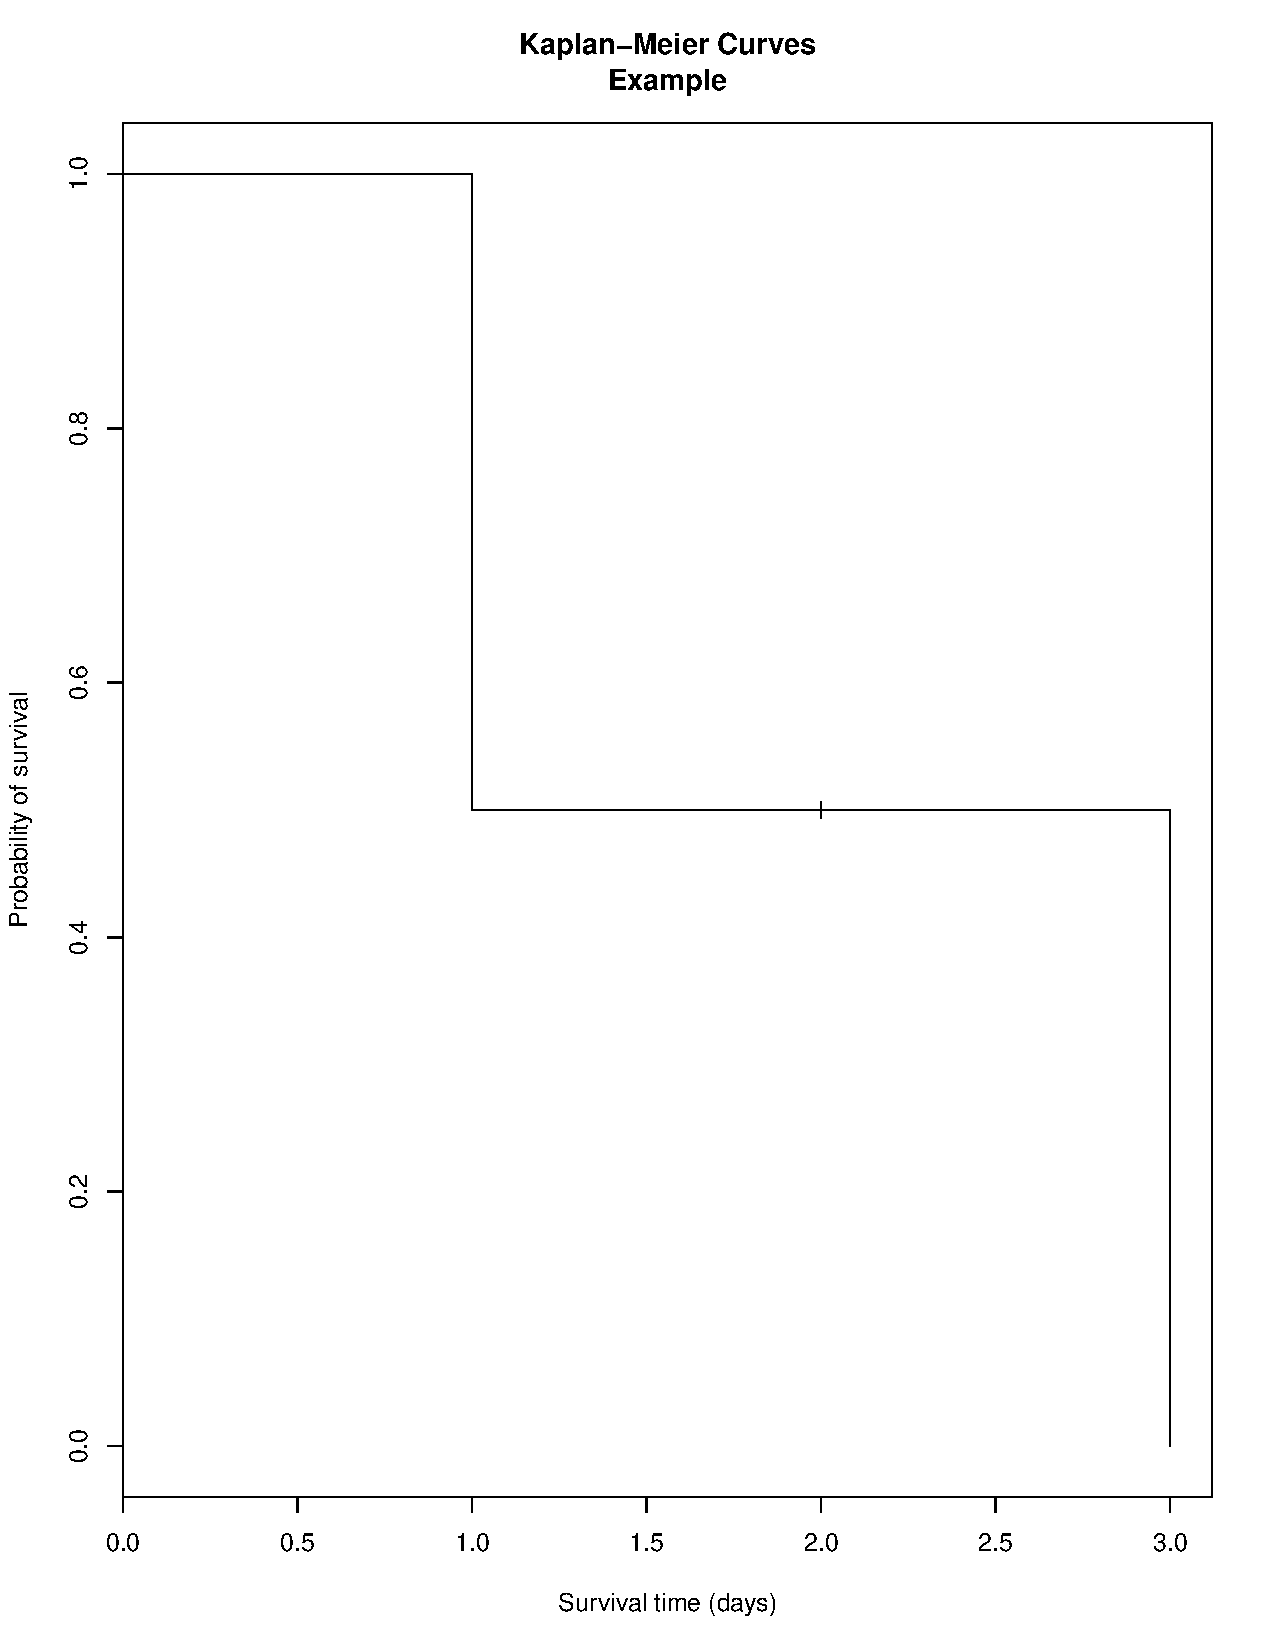
\includegraphics[width=0.5\linewidth,height=4cm]{images/example_survival.pdf}
\caption[Example of survival curve.]{
Example of survival curve for table \ref{survival-example}. Censored data is marked (+) in the plot.}
\end{figure*}



%In analyzing survival data, two functions that are dependent
%on time are of particular interest: the survival function and the
%hazard function.
%The survival function S(t) is defined as the
%probability of surviving at least to time t. The hazard function
%h(t) is the conditional probability of dying at time t having
%survived to that time.

\subsubsection{Comparing survival curves of two groups using the log rank test}

 To compare the survival distributions of two or more groups,  the hypothesis test log-rank test is
 used to test the null hypothesis that there is no difference between the populations
 in the probability of an event at any time point.
%
 The approximated statistics used for comparison purposes for $k$ groups is
 $$T = \sum_{i \in \{1,\ldots,k\}}\frac{(O_i - E_i)^2}{E_i},$$
 where $O_i$ is the observed numbers of death in  group $i$
 while $E_i$ is its expected numbers of deaths.
 If the null hypothesis is true, $T$ is distributed approximately as a $\chi^2_{k-1}$ \cite{matthews1996using}.
If T calculated is $9.44$, and $k = 2$,  evaluating the quantile function (also known as “inverse CDF” or “ICDF”) of the chi-squared distribution the significance level of these data is equal to
$P_r(\chi^2_{1}\geq9.44 = 0.002)$ \cite{yau2012r}.
For a given cut-off, normally $0.05$, the results with p-value smaller are considered significant.

\subsection{Machine Learning}

Machine learning is a field of computer science focused on the development and application of algorithms that improve with experience \cite{mitchell1997machine}.

In genetics and genomics, its  has been applied
 for the interpretation of large genomic data sets and annotation of a wide variety of genomic sequence elements.
For example, for the detection of  transcription start sites (TSSs) locations, which have proven hard to detect in silico due to the complexity and the fairly diffuse structures of Eukaryotic promoters, \citeonline{down2002computational} developped a machine-learning method is able to build useful models of promoters for $>50\%$ of human transcription start sites \cite{down2002computational}.

The machine learning techniques can classified into two main categories: supervised and unsupervised learning (Mitchell, 1997). The supervised learning, which aims to infer data labels by learning from already labeled data, has three stages: design, model and test. The first stage refers to the selection of a learning algorithm used to learn from data (e.g. choose between support vector machines or random forest algoritms) and its training data. The second stage is the creation of a model from labeled data using the algorithm selected priviously.  The last stage uses of this generated model to  preditct the labels of unlabeled data.
The unsupervised learning methods, on the other hand,
cluster the data without using labels, which requires an additional step in which semantics must be manually assigned to each cluster. As this discovery is not tied to previously defined classes, these methods have as benefit the ability to identify potentially novel types of genomic elements.




\subsubsection{Supervised learning}

Supervised learning is a type of machine learning algorithm that identify patterns in data to make predictions.
Specifically, the algorithm takes a known set of input data and known responses to the data (labels), and trains a model to generate predictions for the response to new data.
Supervised learning algorithm can be classified into two  categories: classification and regression.

In classification, the goal is to assign a label to an observation. That is, responses are categorical variables.
For example, given dataset known to be
enhancer or not enhancer, one could want to predict the locations of enhancers in the genome.

In regression, the goal is to predict a continuous measurement for an observation. That is, the responses variables are real numbers. In genomocs, these methods are  used in genetic epidemiology to detect association of genetic variants with a trait or disease of interest \cite{dasgupta2011brief}.




\subsubsection{Unsupervised learning}



%When a labelled training set is not available, unsupervised learning is required. For example, consider the interpretation of a heterogeneous collection of epigenomic data sets, such as those generated by the Encyclopedia of DNA Elements (ENCODE) Consortium and the Roadmap Epigenomics Project. A priori, we expect that the patterns of chromatin accessibility, histone modifications and transcription factor binding along the genome should be able to provide a detailed picture of the biochemical and functional activity of the genome. We may also expect that these activities could be accurately summarized using a fairly small set of labels. If we are interested in discovering what types of label best explain the data, rather than imposing
%a pre-determined set of labels on the data, then we must use unsupervised rather than supervised learning. In this type of approach, the machine learning algorithm uses only the unlabelled data and the desired number of different labels to assign as input.

% In Transcriptomics analysis clustering is used to build groups of genes with related expression patterns

Unsupervised learning is a type of machine learning algorithm used to draw inferences from datasets consisting of input data without labeled responses.
The most common unsupervised learning method is cluster analysis, which is used for exploratory data analysis to find hidden patterns or grouping in data. These algorithms seeks to group a set of objects into cluster (groups) such that those in the same group are more similar to each other than to those in other cluster.
The major unsupervised learning techniques used in bioinformatics are described below.
%In genomics, the Hierarchical clustering, Centroid-based clustering and PCA are commonly used.
\begin{description}

\item[Hierarchical clustering:] {This clustering methods builds a hierarchy of clusters, through either a agglomerative ("bottom up") or a divisive ("top down") procedures.
In the agglomerative procedures, each $n$ observation starts in its own cluster and until only one cluster remains the groups with the smallest dissimilarity are merged.
On the other hand, in the divise procedures, all observations start in one cluster and until all observations are in their own cluster the group is splitted in two groups with biggest dissimilarity. To decide which clusters to merge or divide a metric to measure of dissimilarity between sets of observations is required.
Among the existing agglomerative techniques are the single linkage, also known as the nearest-neighbour technique, which defines the smallest dissimilarity between two points in each group as the dissimilarity between two groups \cite{florek1951liaison}, the complete linkage which defines the largest dissimilarity between two points in each group as the dissimilarity between two groups \cite{defays1977efficient}, the average linkage which defines the average dissimilarity over all points as the dissimilarity between two groups \cite{sokal1958statistical} and the Ward’s method which at each merge step minimizes the increase in the total within-cluster error sum of
squares, which means that  the groups leading to minimum increase in total within-cluster variance are merged \cite{ward1963hierarchical,everitt2011hierarchical}.
The results of hierarchical clustering are usually represented in a dendrogram a branching diagram in which the objects are represented in one of the axis while the similarity between clusters are represented in the other axis by the length of the connection which joins them \cite{manning1999foundations}.}

\item[Optimization clustering
techniques:]{
These are a set of non-hierarchical clustering techniques that cluster individuals into a specified number of groups, by either minimizing or maximizing some numerical criterion \cite{everitt2011hierarchical}.  One of these technique is the k-means algorithms, which iteratively updates a partition by simultaneously relocating each object to the group to whose mean it was closest and then recalculating the group means until the groups no longer change.
More explicitly, let $S = \{S_1,S_2,\ldots,S_k\}$  be the set of k clusters, this algorithms tries to minimize the squared distances of the elements from the cluster center:
$$ N(n,k) = min\sum_{g = 1}^{k}\sum_{j \in S_g}\Vert x_j - \mu_g\Vert^2,$$
where $x_j$ is a data element that belongs to a group g, and $\mu_g$ is the center of points of the $g$ group. A counterpoint of these techniques also requirement to ‘estimate’ the number of clusters in the data, for which a variety of methods
have been suggested and  most are
relatively informal and involve, essentially, plotting the value of the clustering
criterion against the number of groups in which large changes of levels in the plot are
usually taken as suggestive of a particular number of groups.
Some formal methods were also proposed such as the Silhouette index by \citeonline{rousseeuw1987silhouettes}.
And a second counterpoint of this technique is the choice of initial starting values which might lead to local optimal solution, some solution to this problem such as a  bootstrap-like approach to ‘refine’ initial seeds are suggested \cite{steinley2003local}.
}
\item[Principal component analysis (PCA):]{
This method transformes the variables in a multivariate data set into new variables, a linear combination of the original variables, which are uncorrelated with each other and a linear combination of the original variables. This technique provides a means of
projecting the data into a lower dimensional space, which is very useful  mainly due to the problems of high dimensional data which is called ``curse of dimensionality''.
Generally, \citeonline{verleysen2005curse} defines the curse of dimensionality as the expression of all phenomena that appear with high-dimensional data, and that have most often unfortunate consequences on the behavior and performances of learning algorithms. In summary,  the number of learning data should grow exponentially with
the dimension, that means if 10 data  is reasonable to learn a 1-dimensional model, for a 2-dimensional model it will be need 100 data). For example, in genetics, microarray experiments have information for thousand of genes, if each one is considered a variable we would have thousand dimensions,
and we would need an enormous amount of observations to obtain a reliable result. If a dimensionality reduction is not performed, with a increase of data features (dimensions), it is very likely that, by chance, one feature perfectly separates the training examples into positive and negative classes, which would leadto good performance on the training data but poor generalization to data that were not used in training \cite{libbrecht2015machine}.
}
\end{description}

%Another classical and very useful example of unsupervised techniques is the Principal Component Analysis (PCA)
